\begin{figure}[t]
    \centering
    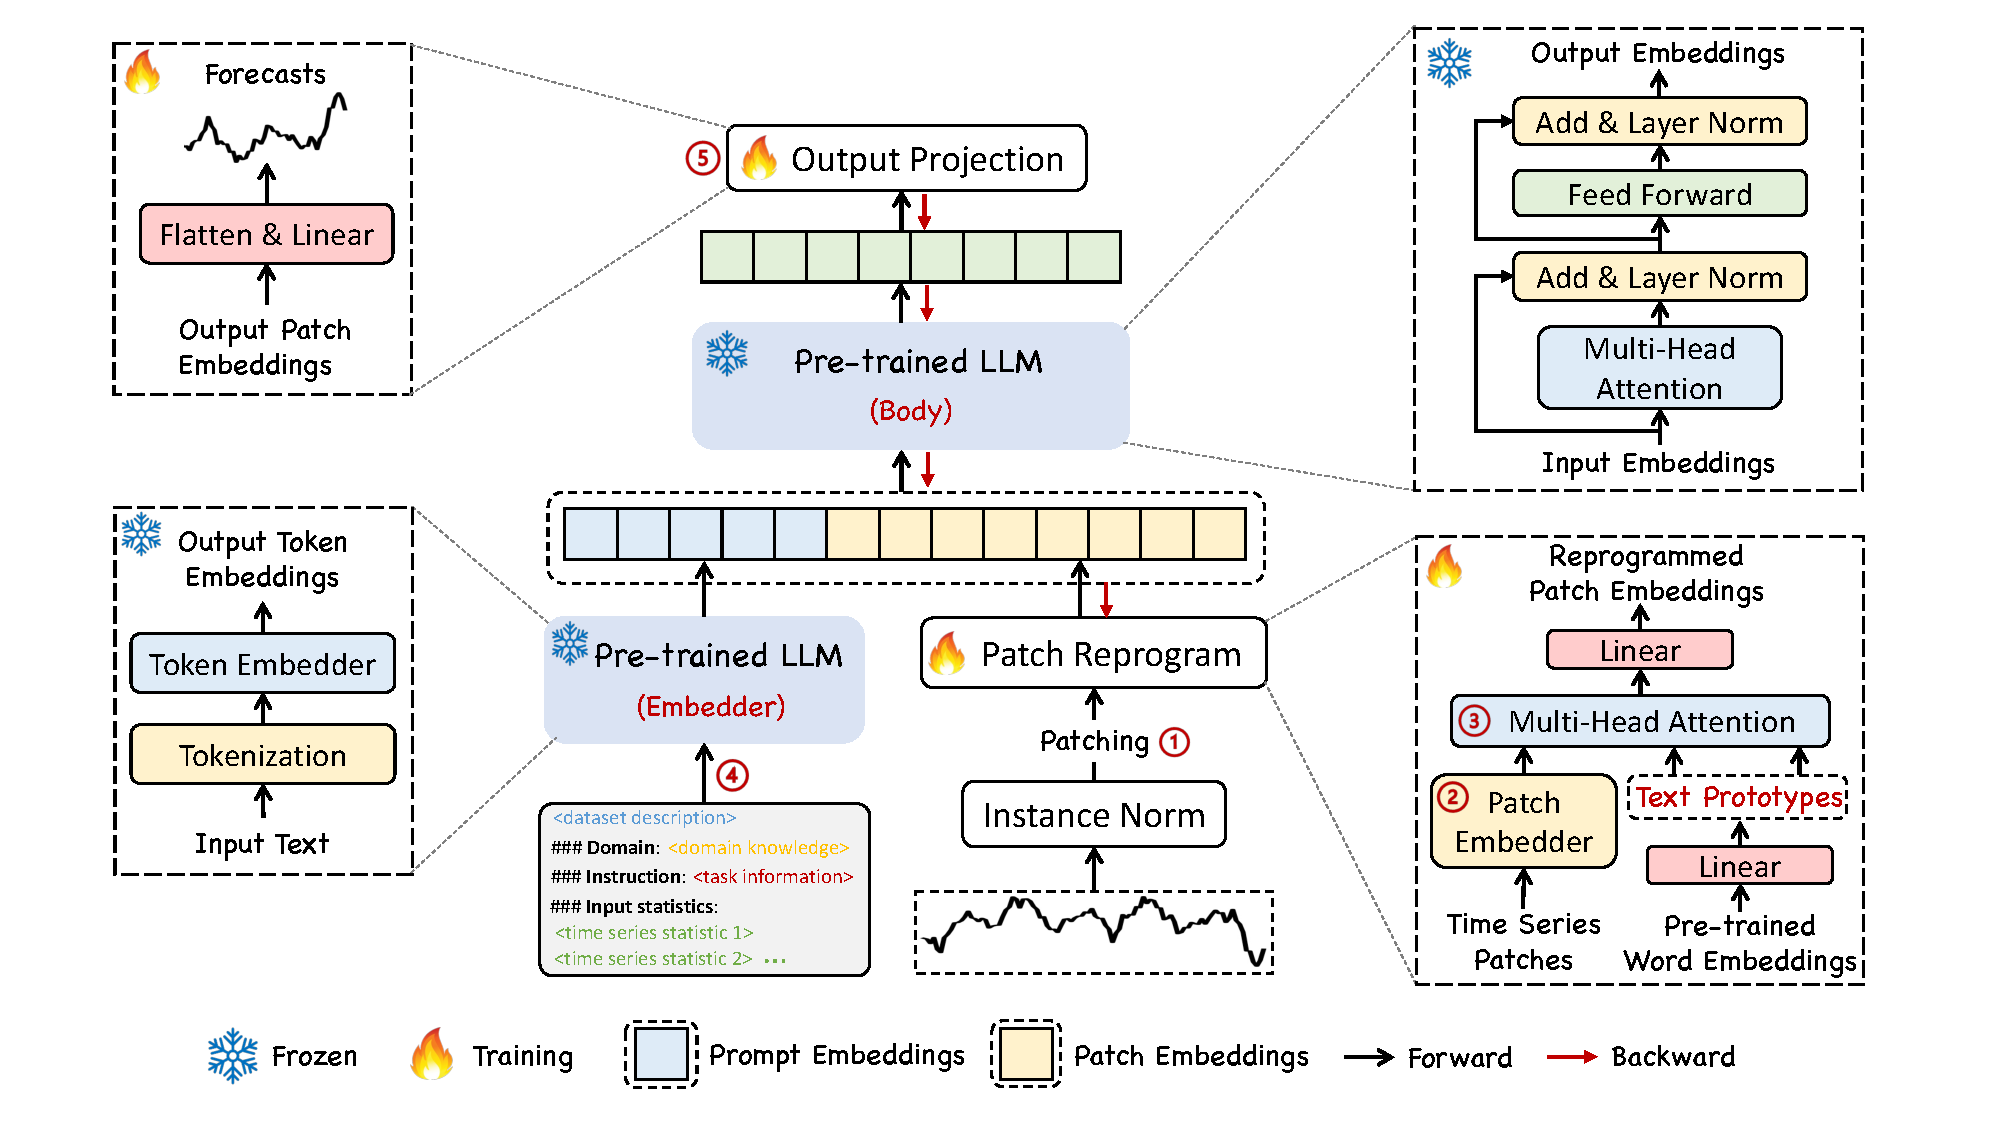
\includegraphics[width=0.95\textwidth]{figures/framework-v4-2.pdf}\vspace{-2mm}
    \caption{
    The model framework of \method. Given an input time series, we first tokenize and embed it via \tikzmarknode[mycircled,red]{a1}{1} patching along with a \tikzmarknode[mycircled,red]{a2}{2} customized embedding layer. \tikzmarknode[mycircled,red]{a3}{3} \revision{These patch embeddings are then reprogrammed with condensed text prototypes to align two modalities.} To augment the LLM's reasoning ability, \tikzmarknode[mycircled,red]{a4}{4} additional prompt prefixes are added to the input to direct the transformation of input patches. \tikzmarknode[mycircled,red]{a5}{5} The output patches from the LLM are projected to generate the forecasts.
    }
    \vspace{-4mm}
    \label{fig:framework}
\end{figure}

Our model architecture is depicted in \shortautoref{fig:framework}. We focus on reprogramming an embedding-visible language foundation model, such as Llama~\citep{touvron2023llama} and GPT-2~\citep{radford2019language}, for general time series forecasting \textbf{\textit{without}} requiring any fine-tuning of the backbone model. Specifically, we consider the following problem: given a sequence of historical observations $\mathbf{X} \in \mathbb{R}^{N \times T}$ consisting of $N$ different 1-dimensional variables across $T$ time steps, we aim to reprogram a large language model $f(\cdot)$ to understand the input time series and accurately forecast the readings at $H$ future time steps, denoted by $\Hat{\mathbf{Y}} \in \mathbb{R}^{N \times H}$, with the overall objective to minimize the mean square errors between the ground truths $\mathbf{Y}$ and predictions, i.e., $\frac{1}{H} \sum_{h=1}^{H} || \Hat{\mathbf{Y}}_h - \mathbf{Y}_h ||^2_F$.

Our method encompasses three main components: (1) input transformation, (2) a pre-trained and frozen LLM, and (3) output projection. Initially, a multivariate time series is partitioned into $N$ univariate time series, which are subsequently processed independently~\citep{nie2022time}. The $i$-th series is denoted as $\mathbf{X}^{(i)} \in \mathbb{R}^{1 \times T}$, which undergoes normalization, patching, and embedding prior to being reprogrammed with learned text prototypes to align the source and target modalities. Then, we augment the LLM's time series reasoning ability by prompting it together with reprogrammed patches to generate output representations, which are projected to the final forecasts $\Hat{\mathbf{Y}}^{(i)} \in \mathbb{R}^{1 \times H}$.

We note that only the parameters of the lightweight input transformation and output projection are updated, while the backbone language model is frozen. In contrast to vision-language and other multimodal language models, which usually fine-tune with paired cross-modality data, \method is directly optimized and becomes readily available with only a small set of time series and a few training epochs, maintaining high efficiency and imposing fewer resource constraints compared to building large domain-specific models from scratch or fine-tuning them. To further reduce memory footprints, various off-the-shelf techniques (e.g., quantization) can be seamlessly integrated for slimming \method.

\subsection{Model Structure}

\noindent\textbf{Input Embedding.}
Each input channel $\mathbf{X}^{(i)}$ is first individually normalized to have zero mean and unit standard deviation via reversible instance normalization (RevIN) in mitigating the time series distribution shift~\citep{kim2021reversible}. Then, we divide $\mathbf{X}^{(i)}$ into several consecutive overlapped or non-overlapped patches~\citep{nie2022time} with length $L_p$; thus the total number of input patches is $P = \lfloor \frac{(T - L_p)}{S} \rfloor + 2$, where $S$ denotes the horizontal sliding stride. The underlying motivations are two-fold: (1) better preserving local semantic information by aggregating local information into each patch and (2) serving as tokenization to form a compact sequence of input tokens, reducing computational burdens. Given these patches $\mathbf{X}^{(i)}_{P} \in \mathbb{R}^{P \times L_p}$, we embed them as $\Hat{\mathbf{X}}^{(i)}_{P} \in \mathbb{R}^{P \times d_{m}}$, adopting a simple linear layer as the patch embedder to create dimensions $d_{m}$.

\noindent\textbf{Patch Reprogramming.} 
Here we reprogram patch embeddings into the source data representation space to align the modalities of time series and natural language to activate the backbone's time series understanding and reasoning capabilities. A common practice is learning a form of ``noise'' that, when applied to target input samples, allows the pre-trained source model to produce the desired target outputs without requiring parameter updates. This is technically feasible for bridging data modalities that are identical or similar. Examples include repurposing a vision model to work with cross-domain images~\citep{misra2023reprogramming} or reprogramming an acoustic model to handle time series data~\citep{yang2021voice2series}. In both cases, there are explicit, learnable transformations between the source and target data, allowing for the direct editing of input samples. However, time series can neither be directly edited nor described losslessly in natural language, posing significant challenges to directly bootstrap the LLM for understanding time series without resource-intensive fine-tuning.

To close this gap, we propose reprogramming $\Hat{\mathbf{X}}^{(i)}_{P}$ using pre-trained word embeddings $\mathbf{E} \in \mathbb{R}^{V \times D}$ in the backbone, where $V$ is the vocabulary size. Nevertheless, there is no prior knowledge indicating which source tokens are directly relevant. Thus, simply leveraging $\mathbf{E}$ will result in large and potentially dense reprogramming space. A simple solution is to maintain a small collection of text prototypes by linearly probing $\mathbf{E}$, denoted as $\mathbf{E'} \in \mathbb{R}^{V' \times D}$, where $V' \ll V$. An illustration is in \shortautoref{fig:framework_details}(a). Text prototypes learn connecting language cues, e.g., ``short up'' (red lines) and ``steady down'' (blue lines), which are then combined to represent the local patch information (e.g., ``short up then down steadily'' for characterizing patch 5) without leaving the space where the language model is pre-trained. This approach is efficient and allows for the adaptive selection of relevant source information. To realize this, we employ a multi-head cross-attention layer.
Specifically, for each head $k = \{1, \cdots, K\}$, we define query matrices $\mathbf{Q}^{(i)}_k = \Hat{\mathbf{X}}^{(i)}_{P} \mathbf{W}^Q_k$, key matrices $\mathbf{K}^{(i)}_k = \mathbf{E'} \mathbf{W}^K_k$, and value matrices $\mathbf{V}^{(i)}_k = \mathbf{E'} \mathbf{W}^V_k$, where $\mathbf{W}^Q_k \in \mathbb{R}^{d_{m} \times d}$ \ and\ \ $\mathbf{W}^K_k, \mathbf{W}^V_k \in \mathbb{R}^{D \times d}$. Specifically, $D$ is the hidden dimension of the backbone model, and $d=\lfloor\frac{d_{m}}{K}\rfloor$.
Then, we have the operation to reprogram time series patches in each attention head defined as:
\begin{equation}
    \mathbf{Z}^{(i)}_k = \textsc{Attention}(\mathbf{Q}^{(i)}_k, \mathbf{K}^{(i)}_k, \mathbf{V}^{(i)}_k) = \textsc{Softmax}(\frac{\mathbf{Q}^{(i)}_k \mathbf{K}^{(i){\top}}_{k}}{\sqrt{d_k}})\mathbf{V}^{(i)}_k.
\end{equation}
By aggregating each $\mathbf{Z}^{(i)}_k \in \mathbb{R}^{P \times d}$ in every head, we obtain $\mathbf{Z}^{(i)} \in \mathbb{R}^{P \times d_m}$. This is then linearly projected to align the hidden dimensions with the backbone model, yielding $\mathbf{O}^{(i)} \in \mathbb{R}^{P \times D}$.

\begin{figure}[t]
    \centering
    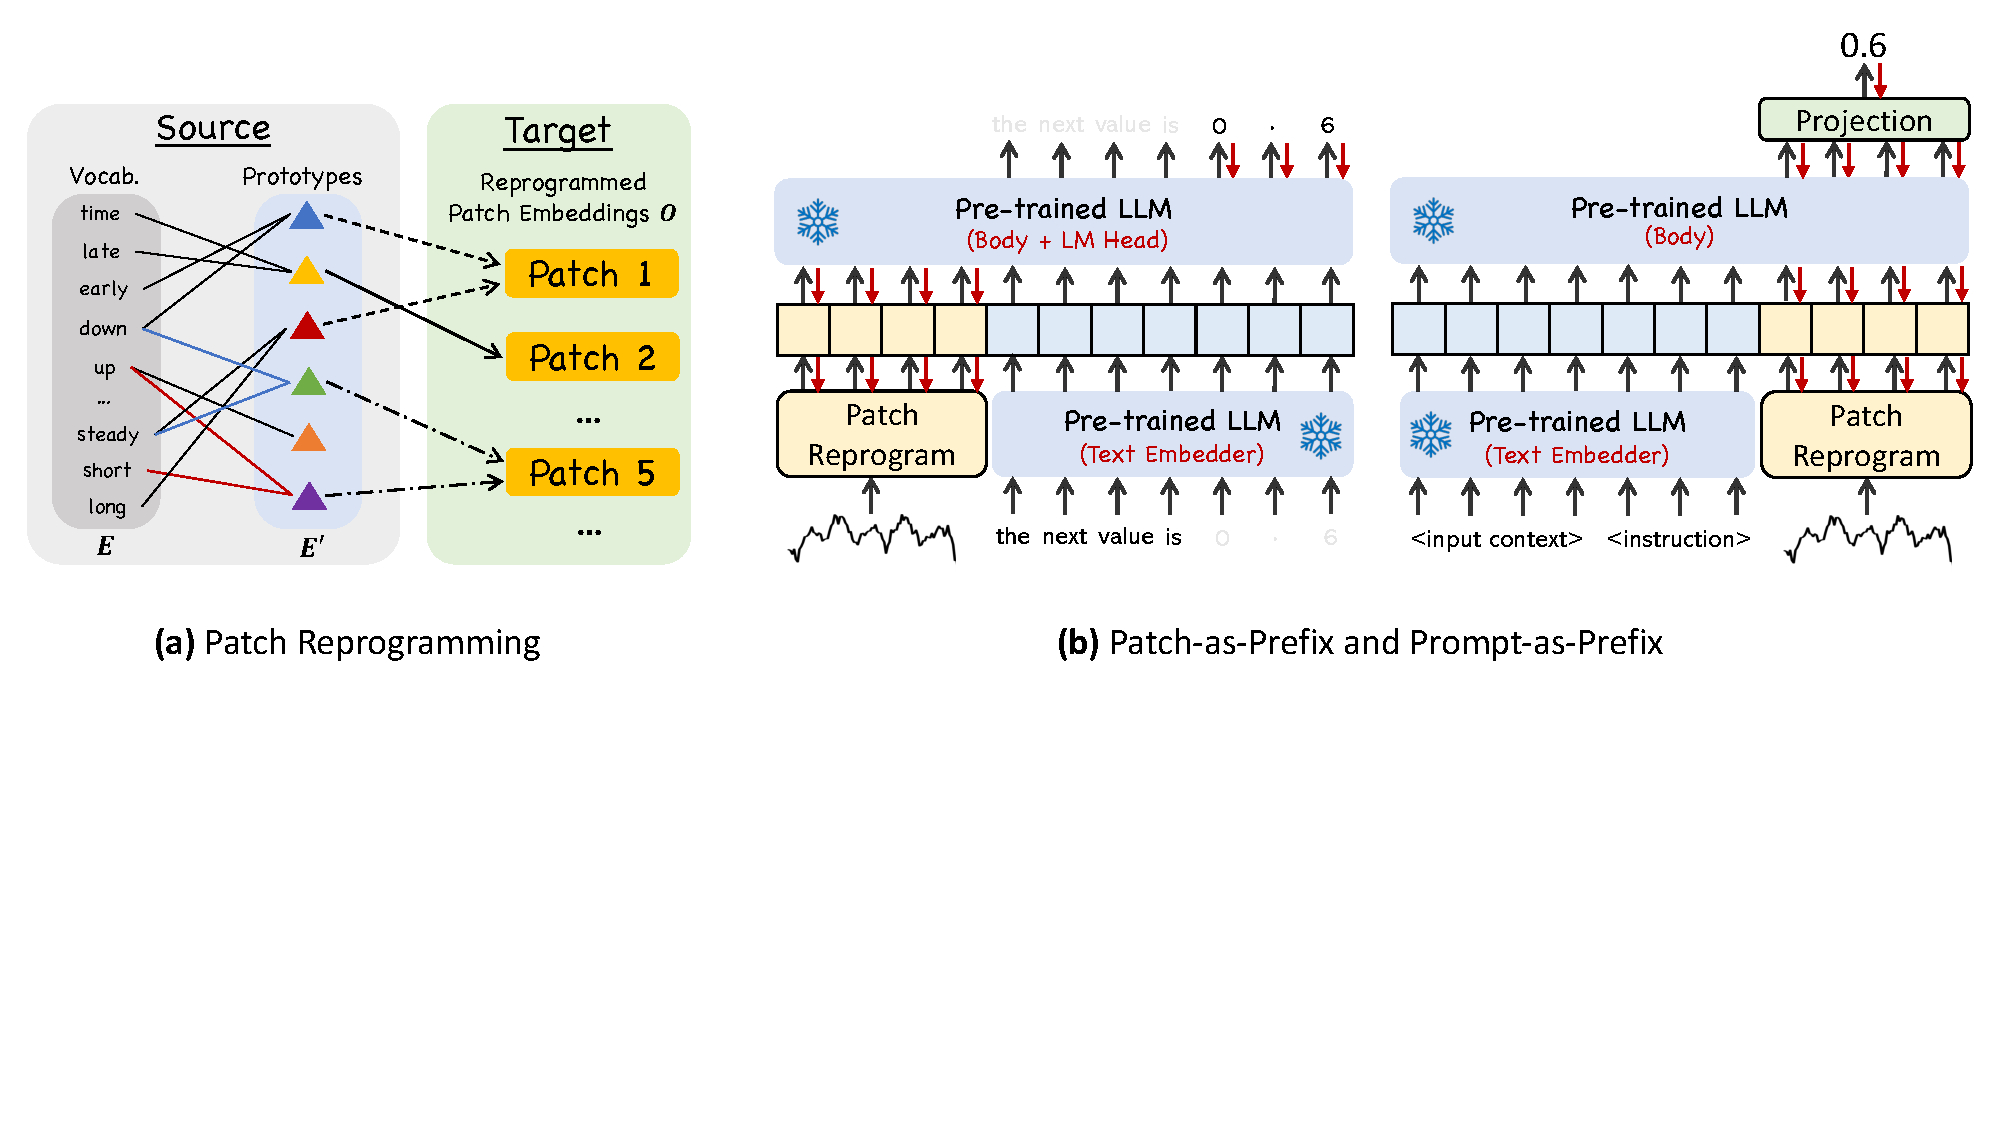
\includegraphics[width=0.99\textwidth]{figures/method-detailed-illustration-v3.pdf}\vspace{-2mm}
    \caption{
    Illustration of \revision{\textbf{(a)} patch reprogramming} and \textbf{(b)} Patch-as-Prefix versus Prompt-as-Prefix.}
    \label{fig:framework_details}
    \vspace{-5mm}
\end{figure}

\begin{wrapfigure}{R}{0.4\textwidth}
\vspace{-3.8mm}
\centering
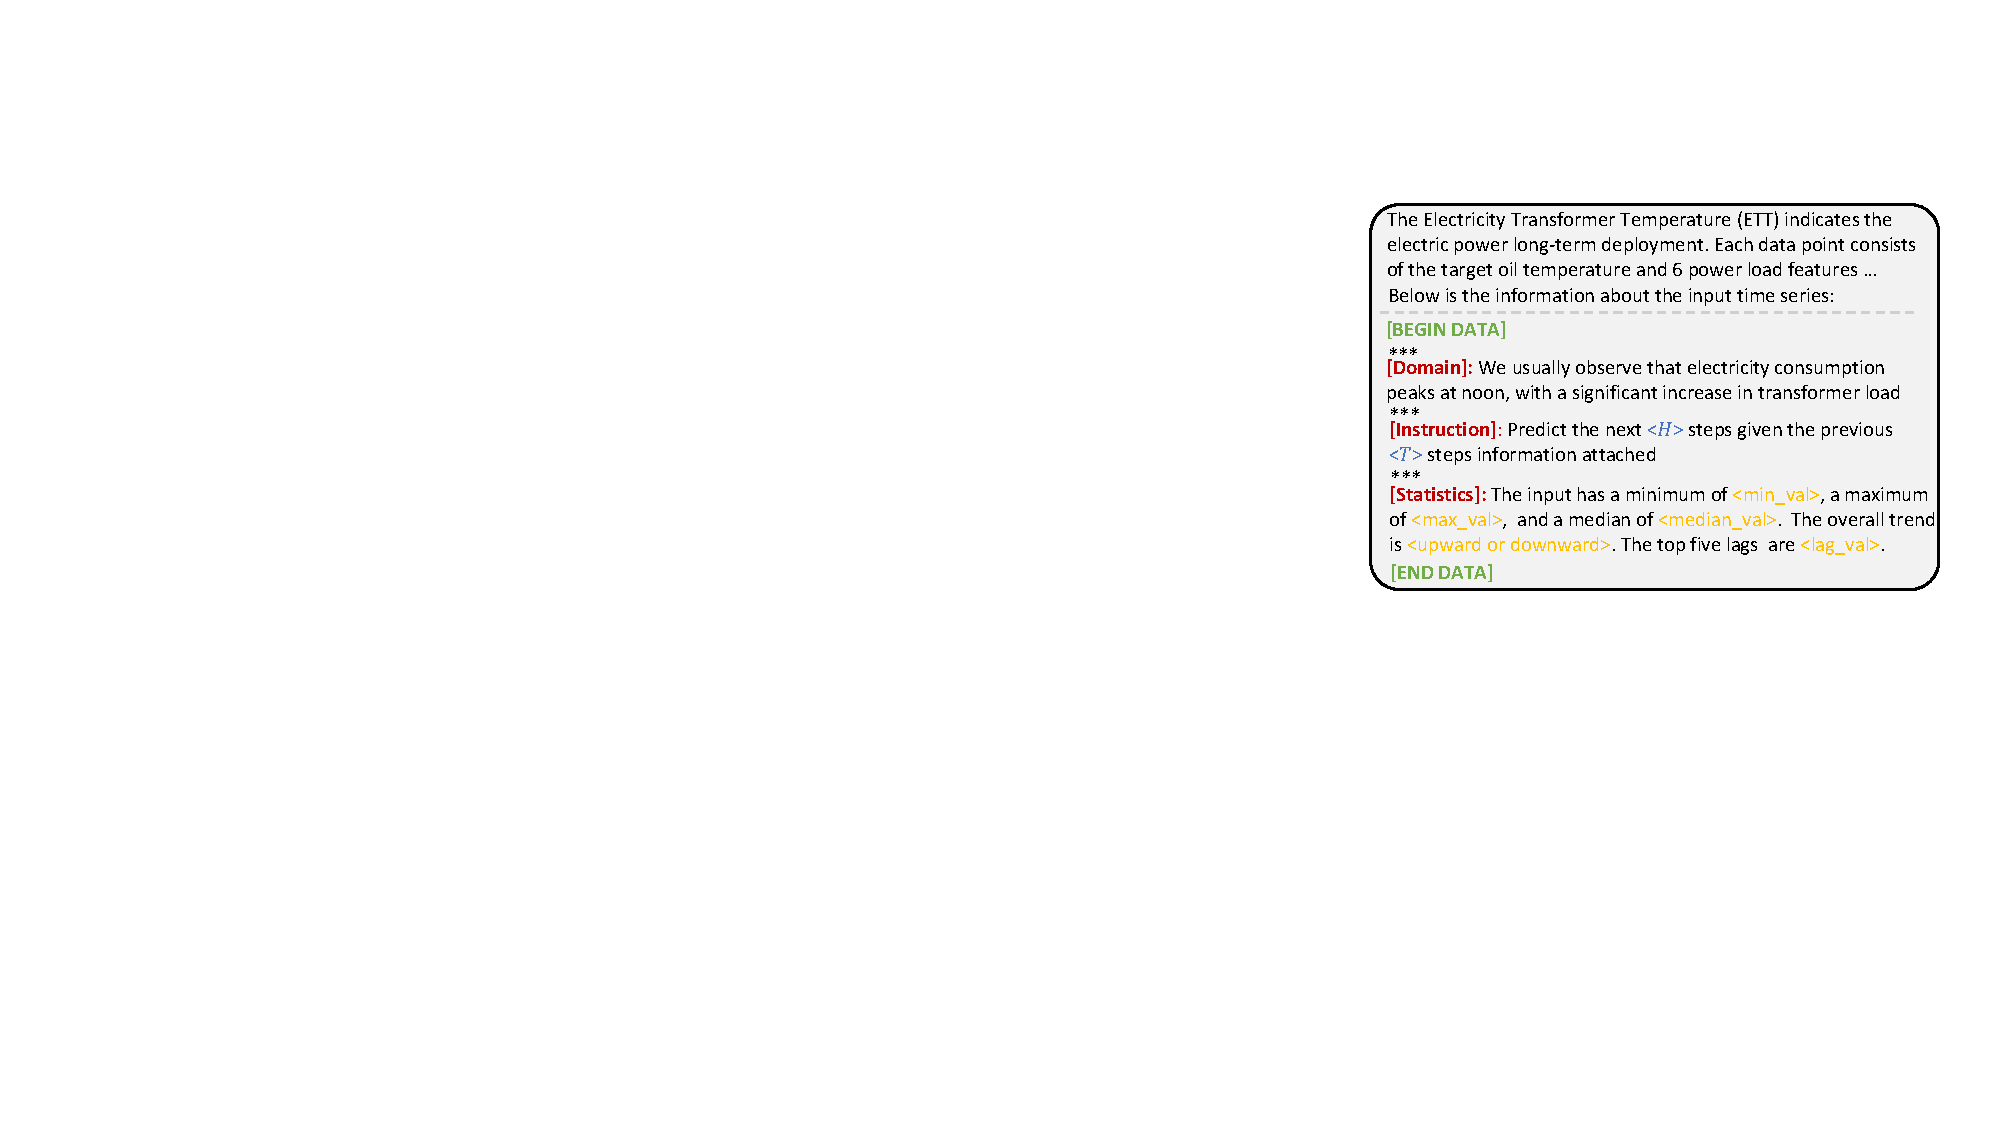
\includegraphics[width=5.8cm]{figures/prompt-example.pdf}
\caption{Prompt example. \textcolor{blue}{$<>$} and \textcolor{orange}{$<>$} are task-specific configurations and calculated input statistics.}
\label{fig:prompt_example}
\vspace{-3.3mm}
\end{wrapfigure}

\noindent\textbf{Prompt-as-Prefix.} 
Prompting serves as a straightforward yet effective approach  task-specific activation of LLMs~\citep{yin2023survey}. However, the direct translation of time series into natural language presents considerable challenges, hindering both the creation of instruction-following datasets and the effective utilization of on-the-fly prompting without performance compromise~\citep{xue2022prompt}. Recent advancements indicate that other data modalities, such as images, can be seamlessly integrated as the prefixes of prompts, thereby facilitating effective reasoning based on these inputs~\citep{tsimpoukelli2021multimodal}. Motivated by these findings, and to render our approach directly applicable to real-world time series, we pose an alternative question: \textit{can prompts act as prefixes to enrich the input context and guide the transformation of reprogrammed time series patches?} We term this concept as \textit{Prompt-as-Prefix} (PaP) and observe that it significantly enhances the LLM's adaptability to downstream tasks while complementing patch reprogramming (See \shortautoref{sec:model_analysis} later).

An illustration of the two prompting approaches is in \shortautoref{fig:framework_details}(b). In \textit{Patch-as-Prefix}, a language model is prompted to predict subsequent values in a time series, articulated in natural language. This approach encounters certain constraints: (1) language models typically exhibit reduced sensitivity in processing high-precision numerals without the aid of external tools, thereby presenting substantial challenges in accurately addressing practical forecasting tasks over long horizons; (2) intricate, customized post-processing is required for different language models, given that they are pre-trained on diverse corpora and may employ different tokenization types in generating high-precision numerals with precision and efficiency. This results in forecasts being represented in disparate natural language formats, such as [`0', `.', `6', `1'] and [`0', `.', `61'], to denote the decimal 0.61.

\textit{Prompt-as-Prefix}, on the other hand, tactfully avoids these constraints.
In practice, we identify three pivotal components for constructing effective prompts: (1) dataset context, (2) task instruction, and (3) input statistics. A prompt example is in \shortautoref{fig:prompt_example}. The dataset context furnishes the LLM with essential background information concerning the input time series, which often exhibits distinct characteristics across various domains. Task instruction serves as a crucial guide for the LLM in the transformation of patch embeddings for specific tasks. We also enrich the input time series with additional crucial statistics, such as trends and lags, to facilitate pattern recognition and reasoning.

\noindent\textbf{Output Projection.}
Upon packing and feedforwarding the prompt and patch embeddings $\mathbf{O}^{(i)}$ through the frozen LLM as shown in \shortautoref{fig:framework}, we discard the prefixal part and obtain the output representations. Following this, we flatten and linear project them to derive the final forecasts $\Hat{\mathbf{Y}}^{(i)}$.